%%%%%%%%%%%%%%%%%%%%%%%%%%%%%%%%%%%%%%%%%
% Propuesta de Desarrollo
% LaTeX Template
% Version 1.0 (06/02/2014)
%
% Original authors:
% Belén Beltran (belubeltran@gmail.com)
% Pablo Ariel Rodriguez (prodriguez@fi.uba.ar)
% Federico Rossi (federicomrossi@gmail.com)
%
%%%%%%%%%%%%%%%%%%%%%%%%%%%%%%%%%%%%%%%%%



%------------------------------------------------------------------------------
%	PACKAGES AND OTHER DOCUMENT CONFIGURATIONS
%------------------------------------------------------------------------------

\documentclass{book}

% Paquetes generales
\usepackage[left=4cm, right=3cm, top=4cm, bottom=3cm, paperwidth=210mm, paperheight=297mm, headsep=1.5cm]{geometry}
\usepackage[utf8]{inputenc}
\usepackage[svgnames]{xcolor} % Required to specify font color
\usepackage{gensymb}

% Paquetes para estilos
\usepackage{textcomp}
\usepackage{setspace}
\usepackage{colortbl}
\usepackage{color}
\usepackage{color}
\usepackage{upquote}
\usepackage{xcolor}
\usepackage{listings}
\usepackage{caption}
\usepackage[T1]{fontenc}
\usepackage[scaled]{beramono}

% Paquetes extras
\usepackage{amssymb}
\usepackage{float}
\usepackage{graphicx}
\usepackage[export]{adjustbox}
\usepackage{url}
\usepackage[toc,page]{appendix}

% Paquete Matematica
\usepackage{mathtools}

% Paquetes para header y footer
\usepackage{fancyhdr}



% Definición de preferencias para la impresión de código fuente.
%% Colores
\definecolor{gray99}{gray}{.99}
\definecolor{gray95}{gray}{.95}
\definecolor{gray85}{gray}{.85}
\definecolor{gray75}{gray}{.75}
\definecolor{gray50}{gray}{.50}



\usepackage{titlesec}

% \titleformat*{\section}{\LARGE\bfseries}
% \titleformat*{\subsection}{\Large\bfseries}
% \titleformat*{\subsubsection}{\large\bfseries}
% \titleformat*{\paragraph}{\large\bfseries}
% \titleformat*{\subparagraph}{\large\bfseries}

% Ocultamos numeración de las secciones
%%\setcounter{secnumdepth}{0}




%------------------------------------------------------------------------------
%	TITLE PAGE
%------------------------------------------------------------------------------

\newcommand*{\titleGM}{\begingroup % Create the command for including the title page in the document
\newcommand*{\sepline}{\color{gray85}\rule[0.5ex]{30em}{0.55pt}}
	
	
\begin{center}

	\vspace*{1.5cm} 

	
\includegraphics[width=9cm]{images/graferator-logo.png} \\[12\baselineskip]

	
	\colorbox{gray95}{
		\parbox[t]{1.0\linewidth}{
			% \centering \fontsize{50pt}{80pt}\selectfont % The first argument for fontsize is the font size of the text and the second is the line spacing - you may need to play with these for your particular title
			\vspace*{0.7cm} % Space between the start of the title and the top of the grey box
			
			\centering {\Huge\bfseries\color{gray50}\fontfamily{fvs}\selectfont Carpeta de Desarrollo}\par % Tagline or further description	
			
			\vspace*{0.7cm} % Space between the end of the title and the bottom of the grey box
		}
	}\\[10\baselineskip]


	% \sepline \\[1\baselineskip]
		\Large Belén Beltran \\
		\large \textit{belubeltran@gmail.com} \\ \medskip
		\Large Pablo Ariel Rodriguez \\
		\large \textit{rodriguez.pabloariel@gmail.com} \\ \medskip
		\Large Federico Martin Rossi \\ 
		\large \textit{federicomrossi@gmail.com} \\

		\bigskip\bigskip

		\large 2do. Cuatrimestre 2014 \\ \smallskip
		\large 75.52 Taller de Programación II \\ \smallskip
		\large Facultad de Ingeniería, Universidad de Buenos Aires \\

\end{center}

	% }}
\endgroup}

\renewcommand{\chaptername}{Capítulo}
\renewcommand{\contentsname}{Contenido}
% \titleformat{\chapter}[display]
%   {\normalfont\bfseries\huge\color{black}}
%   {\chaptertitlename\ \thechapter}{0.5em}{\textbf\Huge} 
% \titleformat{\section}
%   {\normalfont\Large\fontfamily{fvs}\bfseries\color{black}}
%   {\thesection}{1em}{\Large}
% \titleformat{\subsection}
%   {\normalfont\Large\fontfamily{fvs}\color{cyan}}
%   {\thesection}{1em}{\Large}

% \titleformat{\chapter}[hang] 
% {\normalfont\Huge\fontfamily{fvs}}{\chaptertitlename\ \thechapter:}{0.5em}{\Huge} 
% \titleformat{\section}{\normalfont\Large\fontfamily{fvs}}{\thesection}{1em}{\Large}


%% FIGURAS
\captionsetup[figure]{labelfont=bf,textfont=it}
%% TABLAS
\captionsetup[table]{labelfont=bf,textfont=it}

% COMANDOS

%% Titulo de las cajas de código
\renewcommand{\lstlistingname}{Código}
%% Titulo de las figuras
\renewcommand{\figurename}{Imagen}
%% Titulo de las tablas
\renewcommand{\tablename}{Tabla}
%% Referencia a los códigos
\newcommand{\refcode}[1]{\textit{Código \ref{#1}}}
%% Referencia a las imagenes
\newcommand{\refimage}[1]{\textit{Imagen \ref{#1}}}




%------------------------------------------------------------------------------
%	HEADER AND FOOTER
%------------------------------------------------------------------------------


% \pagestyle{fancy}



%------------------------------------------------------------------------------
%	BLANK DOCUMENT
%------------------------------------------------------------------------------

\begin{document}

\pagenumbering{roman}
% \setcounter{page}{0}

% \pagestyle{empty} % Removes page numbers
\thispagestyle{empty}


% This command includes the title page
\titleGM
% \thispagestyle{empty}
% \newpage \textit{}
% \thispagestyle{empty}
% \newpage \textit{}
% \thispagestyle{empty}




% ÍNDICE
\tableofcontents
\newpage
\thispagestyle{empty}
\pagenumbering{arabic}
\thispagestyle{empty}
\thispagestyle{empty}



%
% CAPITULO 1
%
\chapter{Introducción}


% CAPITULO 1
% Descripción general
\section{Descripción general}
	
El presente documento se centra en el desarrollo de \textit{Graferator}, una aplicación de computadora cuyo objetivo es llevar a cabo el estudio de la teoría de grafos con el fin de ser utilizado en la enseñanza y el aprendizaje de la respectiva temática.
\par
Recordando que un grafo es un conjunto conformado por vértices o nodos unidos por enlaces conocidos como aristas o arcos, el software permitirá de manera gráfica la confección y manipulación de estos a través de una interfaz de usuario intuitiva y simple.
\par
Los usuarios podrán hacer uso de dos modalidades de ejecución, a saber:
\medskip

	\begin{itemize}
		\renewcommand{\labelitemi}{\scriptsize\tiny$\blacksquare$} 
		\itemsep=10pt \topsep=0pt \partopsep=0pt \parskip=0pt \parsep=10pt
		
		\item \textbf{Modo edición}: permite editar el grafo agregando nuevos vértices y aristas. 
		
		\item \textbf{Modo aprendizaje}: resolución paso a paso con avance a solicitud del aprendiz (al siguiente paso o al resultado final).

		\item \textbf{Modo autoevaluación}: resolución paso a paso con elaboración guiada del resultado de cada paso a cargo del aprendiz. Confirmación de la corrección del resultado con opción de reintentar en caso de que fuere incorrecto, o ver el resultado correcto.

	\end{itemize}
	\medskip



% CAPITULO 1
% Funcionalidad
\section{Funcionalidad}

Graferactor constará de las funcionalidades básicas que se requieren para el armado de un grafo. Inicialmente se le permitirá al usuario la creación de un \textit{Grafo Orientado} o un \textit{Grafo No Orientado}. 
\par
Además, para cada una de estas opciones se deberá elegir si se desea comenzar a partir de un grafo vacío o si se prefiere generar un grafo aleatorio, especificando la cantidad de vértices y aristas a tomar en cuenta.
\par
De esta manera, la aplicación permitirá:
\medskip

	\begin{itemize}
		\renewcommand{\labelitemi}{\scriptsize\tiny$\blacksquare$} 
		\itemsep=2pt \topsep=0pt \partopsep=0pt \parskip=0pt \parsep=0pt
		
		\item el alta o baja de vértices,

		\item el alta o baja de aristas o arcos,

		\item el borrado del grafo,

		\item la ponderación de arcos.

	\end{itemize}
	\medskip


% CAPITULO 1
% Algoritmos
\section{Algoritmos}

Una vez armado el grafo deseado, Graferator permitirá a los usuarios aplicar sobre este una serie de algoritmos que ayudarán y aportarán al estudio de sus propiedades.
\par
Como se ha adelantado previamente, cada algoritmo podrá ser ejecutado en dos modos distintos (modo aprendizaje y modo autoevaluación). Así, los usuarios no solamente comprenderán el grafo, sino que también adquirirán conocimientos acerca de cómo funcionan los algoritmos aplicables a estos.
\par
De esta manera, habiendo confeccionado el grafo, se podrán efectuar los siguientes algoritmos:


	\begin{itemize}
		\renewcommand{\labelitemi}{\scriptsize\tiny$\blacksquare$} 
		\itemsep=2pt \topsep=0pt \partopsep=0pt \parskip=0pt \parsep=0pt
		
		\item Recorrido en profundidad,

		\item Recorrido en anchura,

		\item Prueba de aciclidad.

	\end{itemize}
	\medskip

	\noindent Si el grafo es orientado, además será posible ejecutar los siguientes:
	\medskip

	\begin{itemize}
		\renewcommand{\labelitemi}{\scriptsize\tiny$\blacksquare$} 
		\itemsep=2pt \topsep=0pt \partopsep=0pt \parskip=0pt \parsep=0pt
		
		\item Recorrido topológico en anchura y en profundidad (si es acícilico),

		\item Obtención de la cerradura transitiva,

		\item Obtención de componentes fuertemente conexas.

	\end{itemize}
	\medskip

	\noindent Si se trata de un grafo orientado con aristas ponderadas:
	\medskip

	\begin{itemize}
		\renewcommand{\labelitemi}{\scriptsize\tiny$\blacksquare$} 
		\itemsep=2pt \topsep=0pt \partopsep=0pt \parskip=0pt \parsep=0pt
		
		\item Algoritmo de caminos mínimos de Dijkstra con un mismo origen (requiriéndose que todas las ponderaciones no sean negativas),

		\item Algoritmo de caminos mínimos de Floyd entre todos los pares de nodos,

		\item Algoritmo de flujos máximos de Ford-Fulkerson.

	\end{itemize}
	\medskip

	\noindent Por último, si el grafo es no orientado:
	\medskip

	\begin{itemize}
		\renewcommand{\labelitemi}{\scriptsize\tiny$\blacksquare$} 
		\itemsep=2pt \topsep=0pt \partopsep=0pt \parskip=0pt \parsep=0pt
		
		\item Algoritmo de árbol de expansión de coste mínimo.

	\end{itemize}
	\medskip



% CAPITULO 1
% Ejecución de algoritmos
\section{Ejecución de algoritmos}

Dispuesto el grafo sobre la zona de diseño y elegido el algoritmo junto con el modo en el cual se ejecutará el mismo, el usuario deberá dar comienzo a la simulación. Para esto la interfaz contará con una serie de controles con los cuales se indicará el inicio o el fin de la ejecución, así como también controles con los que se podrá desplazar a lo largo de esta.
\par
A medida que se corre el algoritmo se podrá visualizar paso a paso la ejecución de este sobre el grafo mediante colores que facilitarán la comprensión del avance en el mismo.
\par
En el momento en que se realiza la elección del algoritmo, habrá una ventana interna en la que se visualizará el pseudocódigo respectivo. En la ejecución se resaltarán una a una las líneas de las sentencias de manera tal que los usuarios realicen un seguimiento detallado de todo el proceso, siendo esto de complemento y apoyo en el aprendizaje del funcionamiento de los distintos algoritmos. A esto se le incluye el conteo del número de sentencias ejecutadas. De esta manera los usuarios tendrán la información necesaria para realizar distintas tareas de análisis, tales como el cálculo de la complejidad algorítmica, refactorización de los algoritmos, entre otros.
\par
Cada paso podrá ser deshecho dado que no solo existirán controles para realizar el avance, sino también para llevar a cabo el retroceso en cualquier instancia del proceso.



%
% CAPITULO 2
%
\chapter{Herramientas de Desarrollo}


% CAPITULO 2
% Lenguaje y entorno de programación
\section{Lenguaje y entorno de programación}

En la presente sección se detallarán aquellas herramientas elegidas para llevar a cabo el desarrollo de la aplicación. 
\bigskip


\subsection{Lenguaje Java}

Se ha optado como lenguaje principal de desarrollo el \textit{Lenguaje Java} versión 1.8. Java es un lenguaje de programación de propósito general,concurrente y orientado a objetos, que fue diseñado específicamente paratener tan pocas dependencias de implementación como fuera posible.
\par
Se ha optado por la utilización de este lenguaje dada la necesidad de queGraferator sea ejecutado al menos en los sistemas operativos MicrosoftWindows y aquellos basados en GNU/Linux. El motivo es que Java ha sido intencionalmente concebido para permitir que los desarrolladores de  aplicaciones escriban programas una única vez y lo ejecuten en cualquier dispositivo (esto se conoce en inglés como WORA o Write Once, Run Anywhere. Es decir, el código que es ejecutado en una plataforma no tiene que ser recompilado nuevamente para poder correr en otra distinta.
\par
Para el desarrollo de esta aplicación se debe contar con la \textit{Java Development Kit 8} la cual se puede descargar de http://www.oracle.com/technetwork/java/javase/downloads/jdk8-downloads-2133151.html
\medskip


\subsection{Eclipse IDE}

Si bien sería posible programar en Java mediante un editor de texto simple, hemos optado por la utilización de un IDE el cual, en nuestro caso será \textit{Eclipse}. Este nos proporciona un ambiente mas ameno para no solo llevar a cabo el desarrollo en sí sino que consigo incluye herramientas de debug, pruebas (JUnit), controladores de versiones, entre otras.
\par
El mismo se puede descargar de https://eclipse.org/downloads/
\medskip


\subsection{WindowBuilder (GUI)}

Para confeccionar la interfaz gráfica se utilizará un plug-in de Eclipse conocido como \textit{WindowBuilder}. Este nos permite desarrollar de forma rápida y cómoda la GUI (interfaz gráfica de usuario) de las aplicaciones Java por medio de una paleta de componentes variados que deben ser arrastrados y soltados sobre un área de diseño. El plug-in se encargará de generar el código necesario para su funcionamiento desligándonos de esta tarea muchas veces engorrosa.
\medskip


\subsection{Maven}

Para mejorar la administración del presente proyecto de software, se ha decidido incorporar el framewor conocido con el nombre de \textit{Maven}. Con administración nos referimos a la gestión el ciclo de vida desde la creación del proyecto hasta la generación del binario que se distribuirá con el proyecto.
\par
Maven es una herramienta que automatiza el proceso de construcción de un proyecto en el lenguaje Java, simplificando enormemente la realización de tareas como borrar los archivos .class, compilar, generar la documentación de javadoc, el jar, generar documentación web, entre otras cosas.
\par
Maven, con comandos simples, crea una estructura de directorios para el proyecto con un sitio para los fuentes, los iconos, ficheros de configuración y datos, etc. Además, nos permite manejar de manera óptima el uso de librerías externas ya que nos permite indicarle qué archivos JARs externos hemos de necesitar y este se ocupará de buscarlos en internet y descargarlos para posteriormente ser incluidos por nosotros.
\par
Provee un conjunto de estándares de construcción, un modelo de repositorio de artefactos y un motor de software que administra y describe los proyectos. Por ejemplo, teniendo en cuenta la naturaleza interdependiente de proyectos open source, Maven permite normalizar ubicaciones para los archivos fuente, documentación y archivos binarios, a fin de proveer una plantilla común para la documentación de proyecto y recuperar dependencias de proyecto de un repositorio compartido, de tal forma que el proceso de construcción consuma menos tiempo y sea mucho más transparente.
\medskip


% CAPITULO 2
% Controlador de versiones
\section{Controlador de versiones}

Para la gestión de los diversos archivos y cambios que puedan surgir sobre estos a lo largo del desarrollo, hemos elegido utilizar el controlador de versiones \textit{Git}. 
\par
Git es un software de control de versiones diseñado por Linus Torvalds, pensando en la eficiencia y la confiabilidad del mantenimiento de versiones de aplicaciones cuando estas tienen un gran número de archivos de código fuente.
\par
Por su parte, hemos optado por utilizar los servicios de Github.com, la cual es una plataforma online de desarrollo colaborativo de software para alojar proyectos utilizando Git. El uso de estos proporcionan varias herramientas útiles que mejoran en gran medida el trabajo en equipo.
\medskip

% CAPITULO 2
% Librerías utilizadas
\section{Librerías utilizadas}
Para el desarrollo de la aplicación se utilizaron las siguientes librerías:
\begin{itemize}
		\renewcommand{\labelitemi}{\scriptsize\tiny$\blacksquare$} 
		\itemsep=10pt \topsep=0pt \partopsep=0pt \parskip=0pt \parsep=10pt
		
		\item \textbf{JGraphT}: Es una librería que permite la representación teórica de un grafo.
		
		\item \textbf{JGraphX}: Es una librería que permite la representación gráfica de un grafo.

		\item \textbf{Log4J}: Es una librería que permite loggear fácilmente información y errores en un archivo. 

	\end{itemize}


% CAPITULO 2
% Herramientas para documentación
\section{Herramientas para documentación}

Por último, para las tareas de documentación y confección de manuales y carpetas hemos decidido utilizar la herramienta \textit{LaTeX}. 
\par
Latex es un sistema de composición de textos, orientado a la creación de documentos escritos que presenten una alta calidad tipográfica. Por sus características y posibilidades, es usado de forma especialmente intensa en la generación de artículos y libros científicos que incluyen, entre otros elementos, expresiones matemáticas. Además, es muy utilizado para la composición de artículos académicos, tesis y libros técnicos, dado que la calidad tipográfica de los documentos realizados es comparable a la de una editorial científica de primera línea.
\par
La realización de los diagramas que componen los documentos se realizarán utilizando la herramienta online \textit{Draw.io}, la cual es comparable con el software Microsoft Visio para la confección de planos y diagramas técnicos.
\par
Finalmente, para el diseño de Mockups de la interfaz gráfica de Graferator, se utilizará la herramienta online \textit{Moqups.com}.



%
% CAPITULO 3
%
\chapter{Diseño de la solución}


% CAPITULO 3
% Estructura general
\section{Arquitectura}

En el primer capítulo de este documento hemos detallado la funcionalidad con la que contara Graferator. Allí hemos podido ver que será necesaria una interfaz gráfica la cual será la mediadora entre el usuario y la aplicación. 
\par
Para contar con un entorno visual va a ser necesario que exista un motor o modelo que lo respalde. Esto es, un módulo que se encarge de manejar aquellos aspectos abstractos e internos que permitirán que el software funcione correctamente. Dado esto es que se cree conveniente utilizar como base en el desarrollo de la aplicación el \textit{patrón de arquitectura Model-View-Controller} o mayormente conocido por sus siglas MVC.
\bigskip

% Imagen 
\begin{figure}[H]
	\centering
	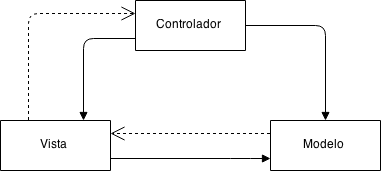
\includegraphics[width=0.6\textwidth]{images/01-MVC.png}
	\medskip
	\caption{Diagrama del patrón de arquitectura MVC}
	\medskip
\end{figure}
	\bigskip
	
El patrón MVC hará posible separar los datos y la lógica de negocio de la interfaz de usuario (también conocida por las siglas GUI) y el módulo encargado de gestionar los eventos y las comunicaciones. Para esto, dicho patrón propone la construcción de tres módulos descentralizados: \textit{Modelo}, \textit{Vista} y \textit{Controlador}. De esta manera, se establecen por un lado los componentes que hacen a la representación de la información y por otro lado se constituyen componentes para la interacción con el usuario. En la \textit{Imagen 3.1} se muestra un diagrama representativo de este patrón.
\par
La totalidad de la aplicación será desarrollada en base a dicha arquitectura en gran medida por los grandes beneficios que significan poseer el modelo y la lógica separados de todo lo restante. Por esta razón, en los siguientes apartados se profundizará sobre cada módulo y se describirán los componentes que lo conforman como así también la forma en la que trabajan entre sí y se comunican con el exterior para lograr los objetivos planteados por el alcance del software.
\newpage


% CAPITULO 3
% Modelo
\section{Modelo}

Como ya se ha adelantado, el \textit{Modelo} es la representación de la información con la cual nuestro sistema operará. Por lo tanto, gestionará todos los accesos a los datos, tanto consultas como actualizaciones. Mediante solicitudes de la \textit{Vista}, este módulo le enviará la información requerida para ser mostrada y visualizada por el usuario. Estas peticiones llegarán al modelo a través del módulo \textit{Controlador}.
\bigskip


\subsection{Componentes básicos}

Primeramente, encontraremos que el modelo necesitará representar a los constituyentes básicos de los grafos. En la \textit{Imagen 3.2} se puede observar un primer diagrama de clases UML en donde se encuentran las clases \textit{Vertice} y \textit{Arista}. Ambas implementarán a la interfaz \textit{Selectable}, quien simplemente establece que tanto los objetos Arista como Vertice son seleccionables. A su vez, Arista hereda de clase que define a objetos con peso, de manera tal que las aristas podrán ser ponderadas cuando así lo requieran.
\par
Por otro lado, la clase Vertice también implementa las interfaces \textit{Serializable} y \textit{Comparable}, las cuales le dan caracteristicas para poder ser serializados y poder ser comparados respectivamente.
\bigskip\bigskip


% Imagen 
\begin{figure}[H]
	\centering
	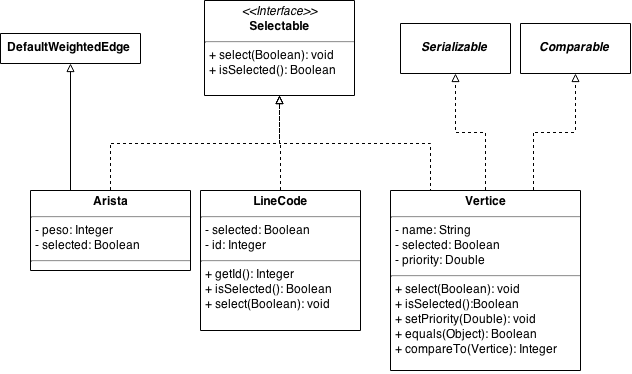
\includegraphics[width=0.95\textwidth]{images/01-01.png}
	\medskip
	\caption{Diagrama de clases de los componentes básicos del modelo}
	\medskip
\end{figure}
\medskip



\subsection{Representación del Grafo}

Conformadas las componentes básicas, necesitamos una entidad que modele al grafo. Esta clase la denominaremos \textit{GraphModel}. Esta hará uso de un conjunto de objetos Vertice relacionados entre sí por objetos del tipo Arista. En la \textit{Imagen 3.3} se puede observar el diagrama de clases en donde se muestra como está conformado GraphModel. Esta clase se relaciona con objetos que implementan la interfaz \textit{Executable}, quien será descrita mas adelante. Además se puede observar que se relaciona con la clase \textit{Resultado}, la cual se encarga de modelar el resultado de aplicar un algoritmo al grafo.
\bigskip\bigskip 


% Imagen 
\begin{figure}[H]
	\centering
	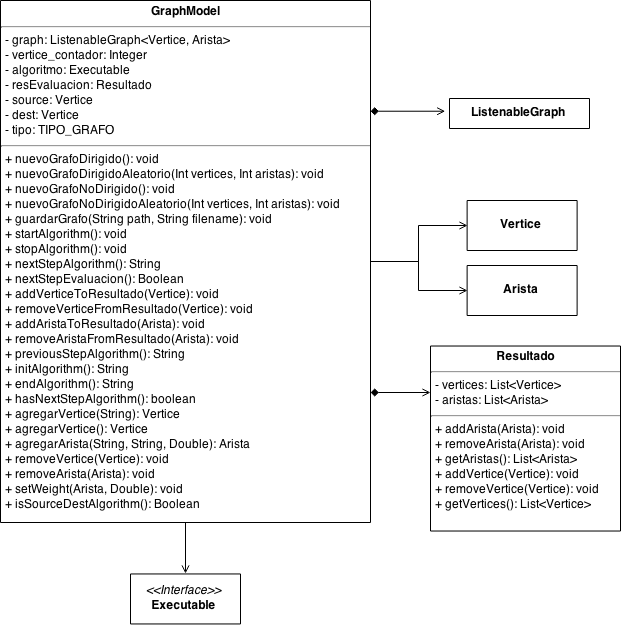
\includegraphics[width=0.8\textwidth]{images/01-03.png}
	\medskip
	\caption{Diagrama de clases de la representación \\ de los grafos.}
	\medskip
\end{figure}
\bigskip



\subsection{Representación de los Algoritmos}

Cada algoritmo mencionado en el Capítulo 1 será representado por una clase del mismo nombre. Todas estas entidades son concretas y heredarán de la clase abstracta \textit{GraphAlgorithm} (\textit{Imagen 3.4}). De esta manera, se hará uso del concepto de polimorfismo utilizado en programación orientada a objetos (OOP) con el fin de no tener un modelo atado a un número fijo de algoritmos, sino que por el contrario, será posible extender la cantidad existente a aplicar sobre los grafos. Por lo tanto, tendremos un modelo altamente escalable.
\bigskip


% Imagen 
\begin{figure}[H]
	\centering
	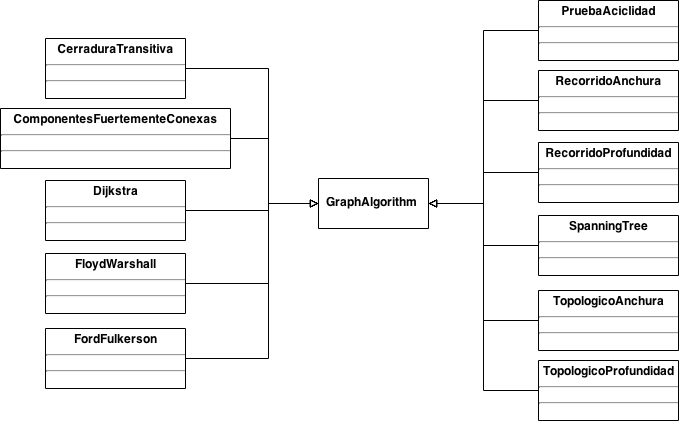
\includegraphics[width=0.8\textwidth]{images/01-04.png}
	\medskip
	\caption{Diagrama de clases con jerarquía de algoritmos.}
	\medskip
\end{figure}
\bigskip

La clase abstracta GraphAlgorithm implementa a su vez las interfaces \textit{Algorithm}, \textit{Documentable} y \textit{Executable}. 
\par
La interfaz Algorithm simplemente permite obtener de aquellas clases que la implementen la URL del archivo en donde se encuentra el pseudocodigo del algoritmo en sí.
\par
Documentable por su parte declara cómo obtener el título y la descripción del algoritmo.
\bigskip


% Imagen 
\begin{figure}[H]
	\centering
	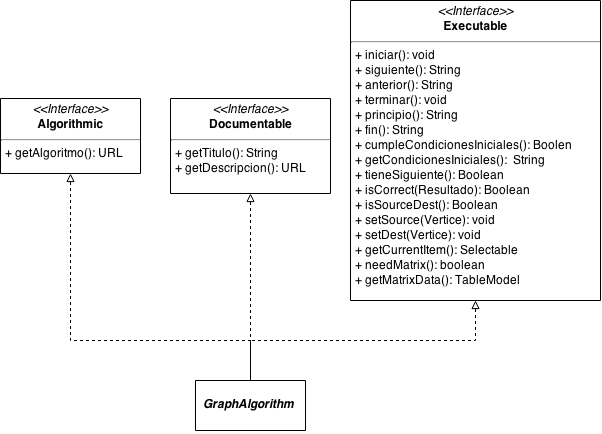
\includegraphics[width=0.70\textwidth]{images/01-02.png}
	\medskip
	\caption{GraphAlgorithm y las interfaces que implementa.}
	\medskip
\end{figure}
\bigskip

Por último, la interfaz Executable establece los métodos a través de los cuales se podrá ejecutar el algoritmo. Este fuerza a declarar y definir los métodos que permiten iniciar y detener la ejecución, como así también avanzar y retroceder en cualquier punto de la corrida. Además declara mensajes especiales para comunicarse con los algoritmos, como por ejemplo, \textit{isCorrect()}, al cual se le deberá pasar como parámetro un objeto del tipo Resultado y el algoritmo responderá si, en el paso actual, el resultado concuerda con este último. En la \textit{Imagen 3.5} se muestra el diagrama correspondiente a lo recién descrito.
\bigskip


% CAPITULO 3
% Vista
\section{Vista}

\subsection{Mockups}

Para el desarrollo de la vista se ha utilizado, como ya se ha mencionado en el Capítulo 2, el diseñador de GUIs de Java \textit{WindowBuilder}. Nos limitaremos aquí a mostrar los distintos mockups que definirán la interfaz gráfica de Graferator.
\par
En la \textit{Imagen 3.6} se puede observar la pantalla inicial que verán los usuarios al iniciar la aplicación. Inicialmente no se abrirá ninguna ventana. Se contará con un menú superior donde se encontrarán las opciones de inicialización. Allí se podrá crear un grafo orientado o no orientado vacío, como así también se encontrará la opción de crear un grafo aleatorio de estos mismos tipos. En este mismo menú se encontrarán las opciones de guardar y abrir, cuya funcionalidad se orienta a poder persistir el grafo creado por los usuarios para abrirlo y utilizarlo en un futuro.
\bigskip

% Imagen 
\begin{figure}[H]
	\centering
	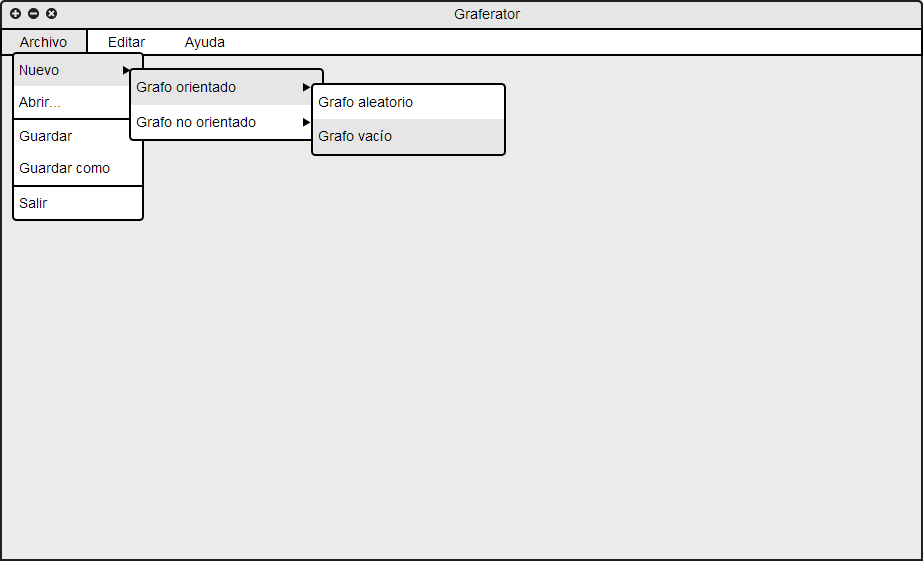
\includegraphics[width=0.9\textwidth]{images/02-01.png}
	\medskip
	\caption{Mockup de la ventana inicial de Graferator}
	\medskip
\end{figure}
\bigskip

Una vez elegido el tipo de grafo con el que se desea trabajar, se habilitarán las distintas ventanas internas que conforman el entorno del software (\textit{Imagen 3.7}). Este último estará conformado por un panel izquierdo cuya zona superior contendrá un listado de los algoritmos disponibles dispuestos con radio buttons forzando a que solo pueda ser elegido uno a la vez. En la zona inferior se podrá elegir el modo con el que se ejecutará el algoritmo (modo aprendizaje, modo autoevaluación y modo edición).
\newpage
A la derecha se encontrará un panel con dos pestañas: \textit{Información} y \textit{Algoritmo}. En la pestaña Información se podrán visualizar datos generales referentes al algoritmo activo (historia, particularidades, etcétera). En cambio, en la pestaña Algoritmo se encontrará el pseudocódigo correspndiente con La particularidad de que al iniciar la ejecución y avanzar o retroceder, los usuarios tendrán a disposición la línea del pseudocódigo activa resaltada con color. Esto permitirá un seguimiento mas ilustrativo de todo el proceso de análisis y estudio.

En la parte superior central, justo debajo de la barra de menú, se encontrará la barra de control. Esta barra contendrá los controles necesarios para llevar a cabo la ejecución de los algoritmos, es decir, tendrá los botones de \textit{Iniciar}, \textit{Avanzar}, \textit{Retroceder}, \textit{Ir al final} y \textit{Volver al inicio}.
\bigskip

% Imagen 
\begin{figure}[H]
	\centering
	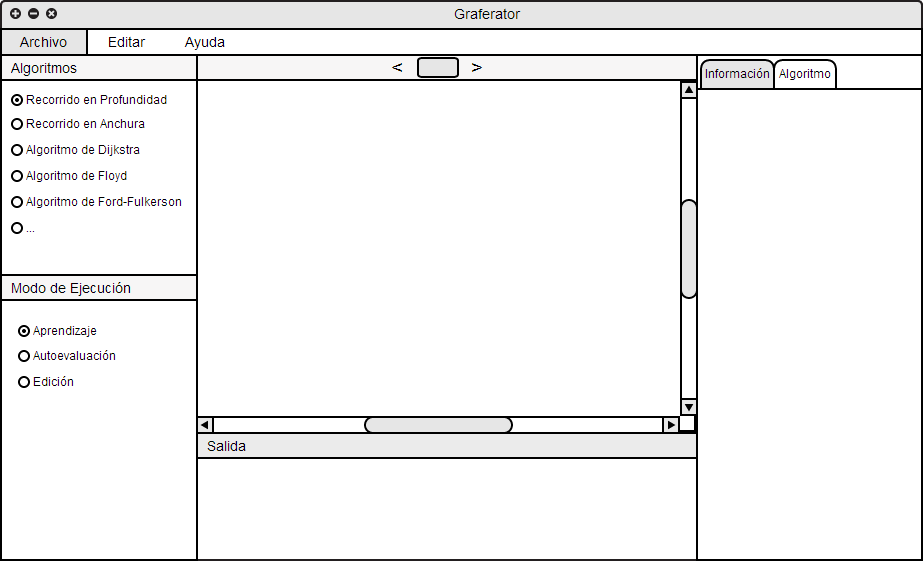
\includegraphics[width=0.9\textwidth]{images/02-02.png}
	\medskip
	\caption{Mockup de la distribución de ventanas internas \\ sobre el entorno.}
	\medskip
\end{figure}
\bigskip

Se poseerá además, en la parte inferior, una ventana de salida en donde se podrán leer los resultados o mensajes provenientes de la ejecución y de los propios algoritmos. Allí se visualizarán los resultados finales de ejecución con formatos legibles y podrán ser fácilmente copiados para su utilización en medios externos a Graferator.
\par
Por último, ubicado en el centro de la ventana central se encuentra la zona de trabajo principal. Allí los usuarios deberán confeccionar el grafo deseado. Para esto tendrán que hacer uso del menú editar de la barra superior, en donde encontrarán las opciones para agregar nuevos vértices y aristas. Luego podrán posicionar estos sobre dicha área para su posterior ejecución.
\newpage

% Imagen 
\begin{figure}[H]
	\centering
	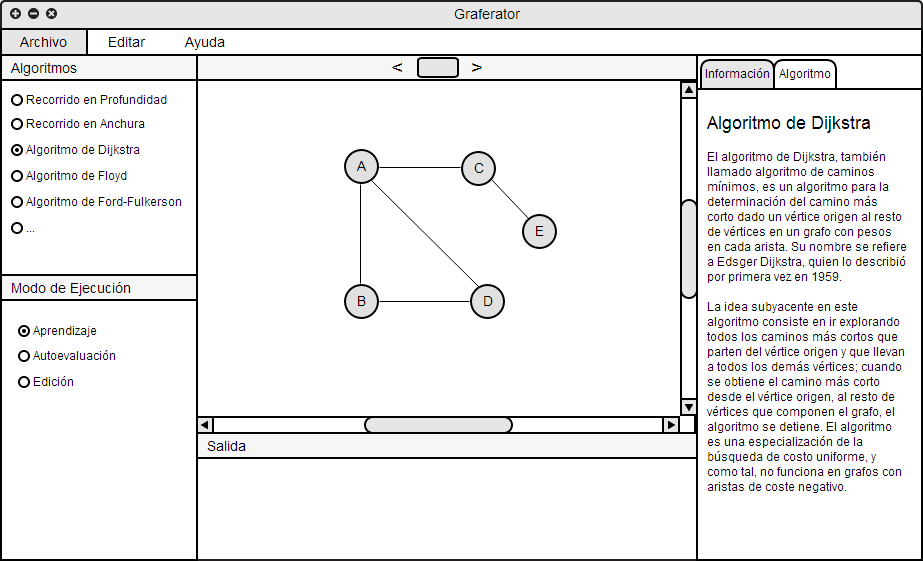
\includegraphics[width=0.9\textwidth]{images/02-03.png}
	\medskip
	\caption{Mockup del área de trabajo en donde \\ se diseñarán los grafos.}
	\medskip
\end{figure}
\bigskip



\subsection{Diagramas de Clases}

En cuanto se refiere al diseño de la vista en sí podemos destacar las siguientes clases importantes:
\medskip

	\begin{itemize}
		\renewcommand{\labelitemi}{\scriptsize\tiny$\blacksquare$} 
		\itemsep=10pt \topsep=0pt \partopsep=0pt \parskip=0pt \parsep=10pt
		
		\item \textbf{Main}: Contiene los componentes generales.
		
		\item \textbf{GraphView}: Contiene la representación gráfica del grafo. 
		
		\item \textbf{PanelAlgoritmos}: Contiene los botones de selección de algoritmos.
		
		\item \textbf{PanelInformación}: Contiene la información de los algoritmos.
		
		\item \textbf{PanelModo}: Contiene los botones de selección de modo.
		
		\item \textbf{PanelPseudocódigo}: Contiene el pseudocódigo de los algoritmos.
		
		\item \textbf{PapersMenu}: Contiene el menú de la aplicación.
		
		\item \textbf{PapersToolbar}: Contiene los botones de Inicio/Fin, siguiente y atrás de la ejecución de los algoritmos.

	\end{itemize}
	\medskip

Las relaciones entre las mismas se detallan en la \textit{Imagen 3.9}.

\newpage

% Imagen 
\begin{figure}[H]
	\centering
	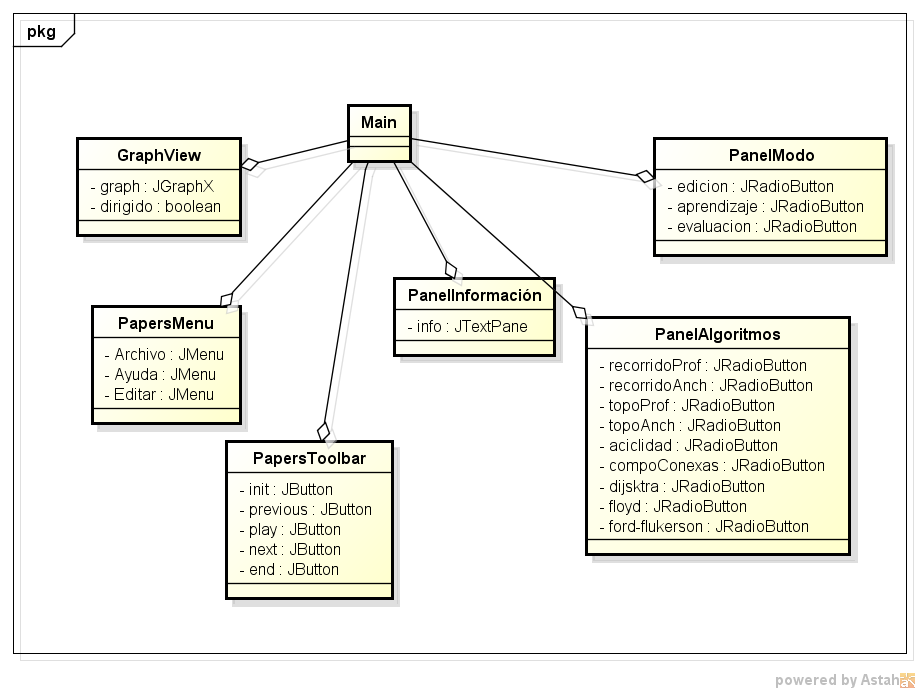
\includegraphics[width=1\textwidth]{images/vista.png}
	\medskip
	\caption{Diagrama de clases de la Vista.}
	\medskip
\end{figure}
\bigskip

\newpage
% CAPITULO 3
% Controlador
\section{Controlador}

El módulo Controlador contiene las clases que gestionan las acciones del usuario (selección de algoritmos, modo, creación de aristas, etc.) y es el encargado de reflejar dichas acciones tanto en modelo como en la vista.
\medskip

\subsection{Listeners del Menú}

Son las clases que contienen la gestión de las acciones de los diferentes menús.
Las relaciones entre las mismas se detallan en la \textit{Imagen 3.10}.
% Imagen 
\begin{figure}[H]
	\centering
	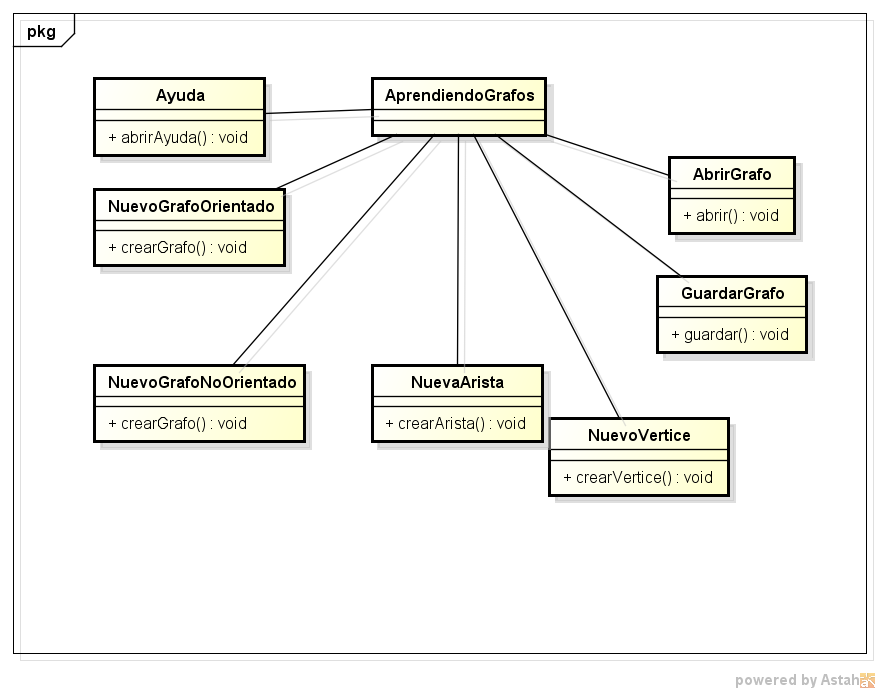
\includegraphics[width=1\textwidth]{images/menu.png}
	\medskip
	\caption{Diagrama de clases de los listeners del Menú.}
	\medskip
\end{figure}
\bigskip

\subsection{Listeners del Mouse}

Son las clases que contienen la gestión de las acciones realizadas con el Mouse (selección de vértices, creación de vértices y aristas, etc.).
Las relaciones entre las mismas se detallan en la \textit{Imagen 3.11}.
% Imagen 
\begin{figure}[H]
	\centering
	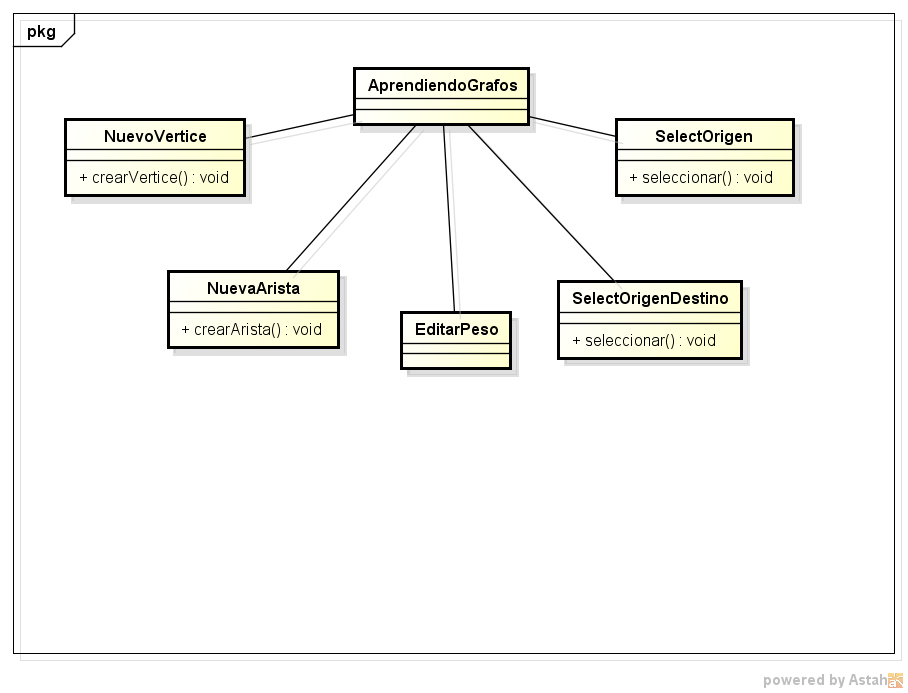
\includegraphics[width=0.6\textwidth]{images/mouse.png}
	\medskip
	\caption{Diagrama de clases de los listeners del mouse.}
	\medskip
\end{figure}
\bigskip

\subsection{Listeners de ejecución}

Son las clases que contienen la gestión de las acciones que conciernen a la ejecución de los algoritmos (siguiente, atrás, inicio/fin, etc.).
Las relaciones entre las mismas se detallan en la \textit{Imagen 3.12}.
% Imagen 
\begin{figure}[H]
	\centering
	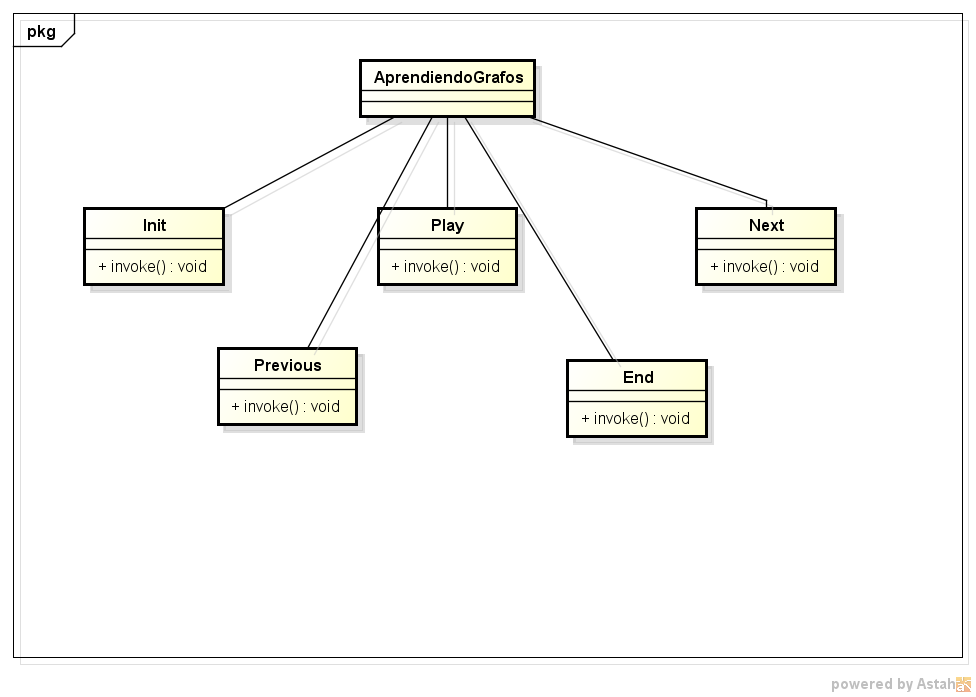
\includegraphics[width=0.9\textwidth]{images/ejecucion.png}
	\medskip
	\caption{Diagrama de clases de los listeners de ejecución}
	\medskip
\end{figure}
\bigskip
\newpage



\end{document}